\begin{frame}{What is this thesis about?}
\begin{block}{}
\begin{itemize}
\item A sparsely sampled light field reconstruction method of a static scene. 

\bigskip
\pause
\item This method uses Universal Shearlets to perform an inpainting algorithm in the sparse Epipolar planes images (EPIs).

\bigskip 
\pause
\item The EPIs are images with linear structures obtained by tracking different feature points in a sequence of pictures of the scene. 

\bigskip
\pause
\item The slope of the straight lines in the EPIs can be used to compute the depth of feature points in the scene and therefore the depth map that contains the 3D information of the scene.

\bigskip
\pause
\item The thesis presents all the steps in the reconstruction pipeline with theory, algorithms and code. 
\end{itemize} 
\end{block}
\end{frame}

\begin{frame}{Involved concepts}
\begin{block}{}
\begin{itemize}
\item Early Vision (biology) and Light Field Theory (physics).

\bigskip
\pause
\item Computer Vision for point tracking and line detection (basic concepts of linear algebra).

\bigskip 
\pause
\item Functional Analysis and Computational Harmonic Analysis (sparsifying dictionaries).

\bigskip
\pause
\item Compressed sensing techniques ($\ell^1$ optimization algorithms). 
\end{itemize}
\end{block}
\end{frame}

\begin{frame}{Light Field Thoery}
\begin{block}{}
\begin{itemize}

\item In 1846 Michael Faraday proposed for the first time on his lecture "Thoughts on Ray Vibration" that light could be interpreted as a field.

\pause

\item Propagation of light rays in the 3D space is completely described by a 7D continuous function $L(x,y,z,\theta,\phi, \lambda, \tau)$ called the plenoptic function

\pause
\begin{figure}[h!]
\centering
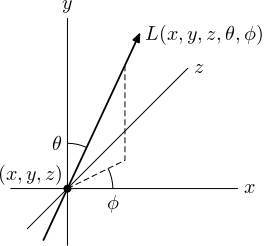
\includegraphics[width=0.25\textwidth]{../../Diagrams/Plenoptic_function.jpg}
\end{figure}

\pause

\item The plenoptic function can be simplified to a 4D function $L_4$, called 4D Light Field or simply Light Field, which quantifies the intensity of static and monochromatic light rays propagating in half space. 
\end{itemize}
\end{block}
\end{frame}

\begin{frame}{4D Light Field Representation}
\begin{figure}[h!]
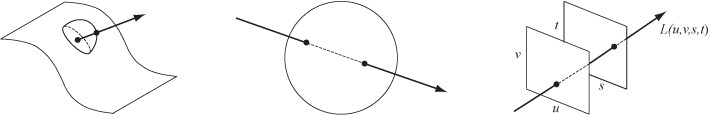
\includegraphics[width=0.8\textwidth]{../../Diagrams/Light-field-parametrizations.jpg}
\caption{Three different representation of 4F LF\@. Left: $L_4(u,v,\phi,\theta)$. Center: $L_4(\phi_1,\theta_1,\phi_2,\theta_2)$. Right: $L_4(u,v,s,t)$.}
\end{figure}
\pause
\begin{figure}[h!]
\centering
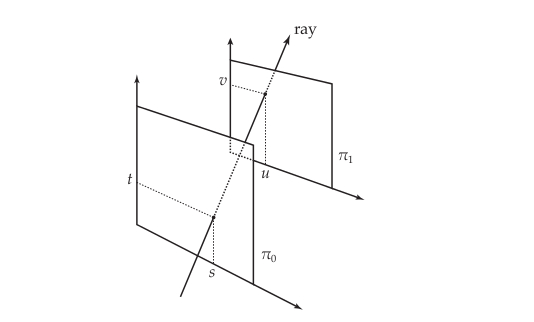
\includegraphics[width=0.5\textwidth]{../../Diagrams/two-planes_param.jpg}
\caption{Used representation: "Two plane parametrization".}
\label{fig:C2S0F3}
\end{figure}
\end{frame}

\begin{frame}{}

\begin{center}
\textbf{\huge{Motivation}}
\end{center}

\end{frame}


\begin{frame}{Compression of High Resoluation Light Field (Wetzstein et al., 2013)}
\begin{figure}[h!]
\centering
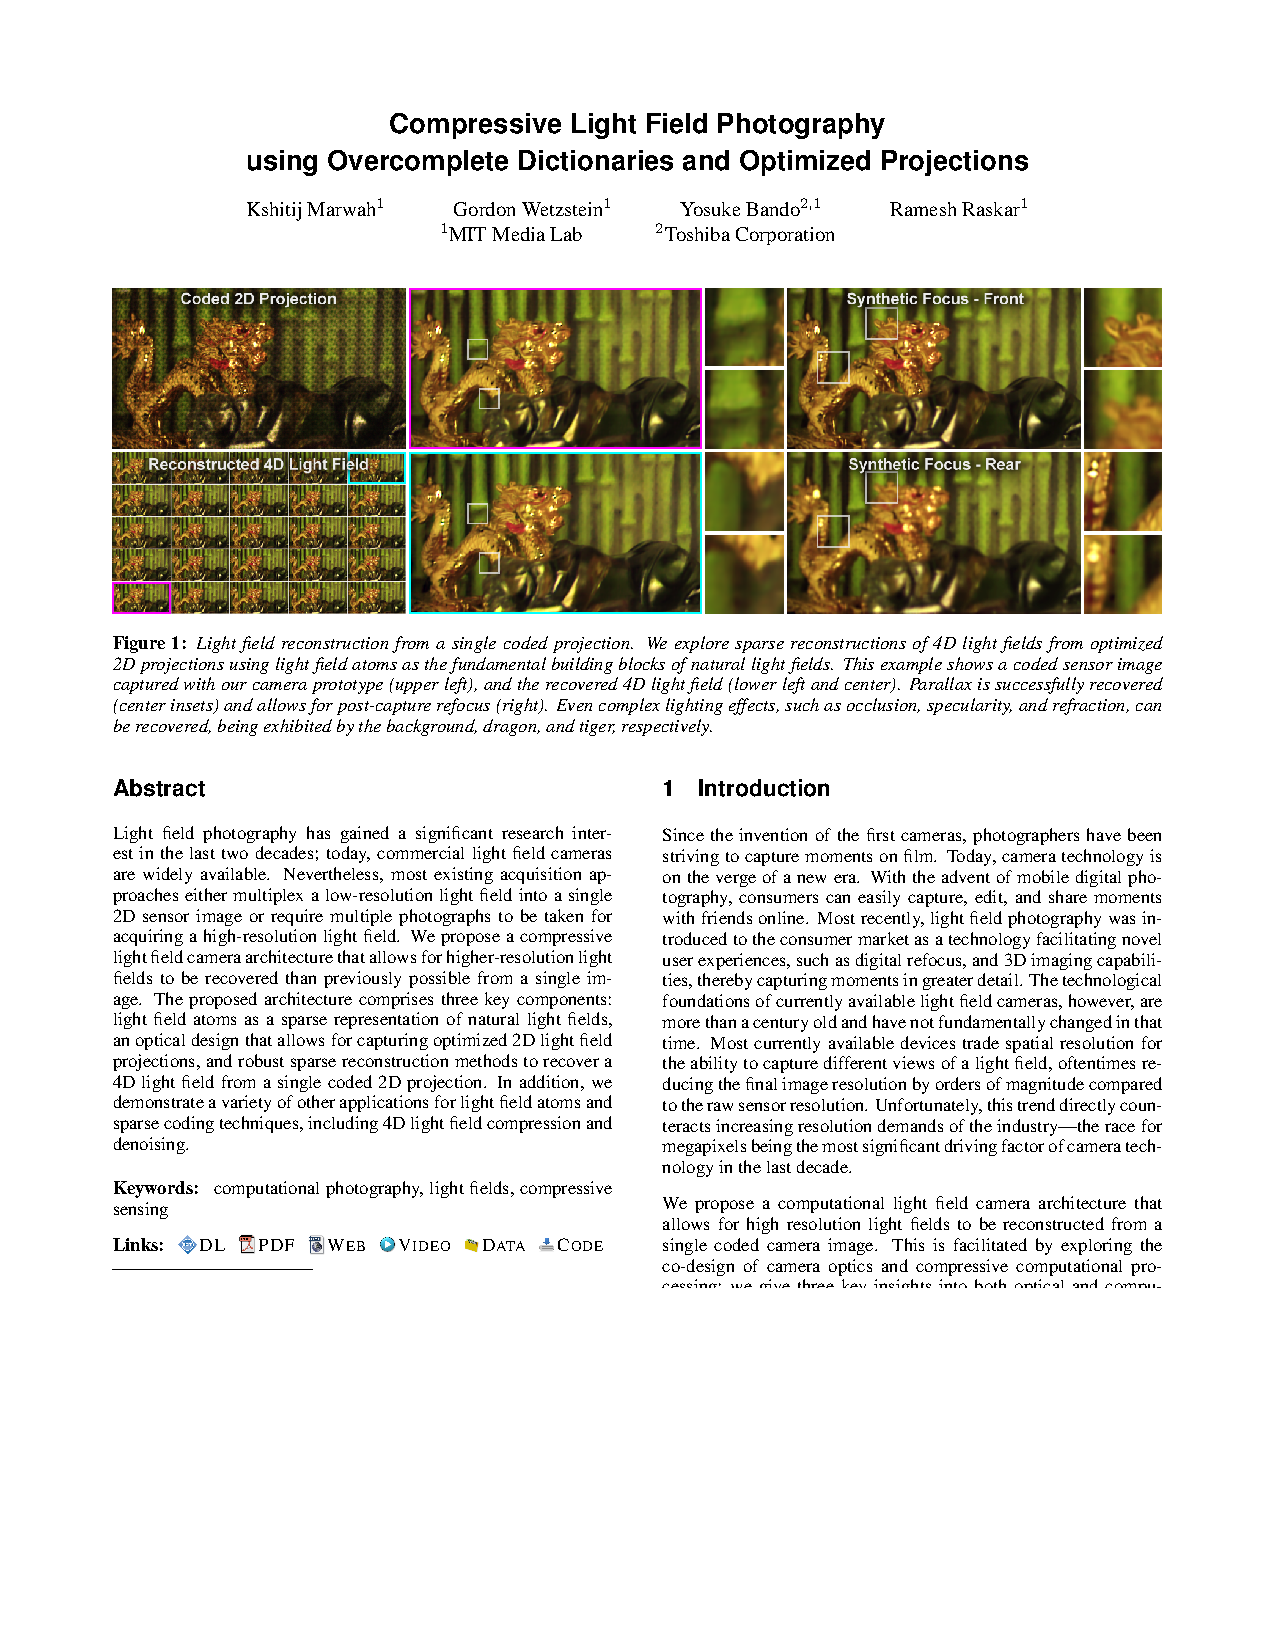
\includegraphics[width=0.7\textwidth]{./images/compressed_light_field.pdf}
\label{fig:C2S0F3}
\end{figure}
\end{frame}

\begin{frame}{Raytrix (Perwass and Wietzke, 2010)}
\begin{figure}[h!]
\centering
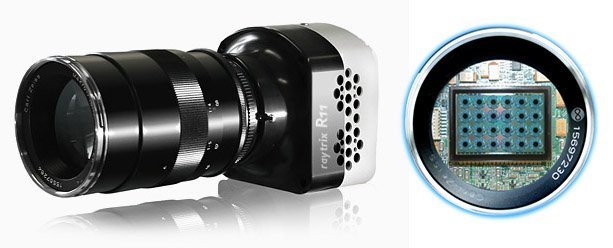
\includegraphics[width=1\textwidth]{../../Diagrams/raytrix.jpg}
\label{fig:C2S0F3}
\end{figure}
\end{frame}

\begin{frame}{Lytro (Ng, 2012)}
\begin{figure}[h!]
\centering
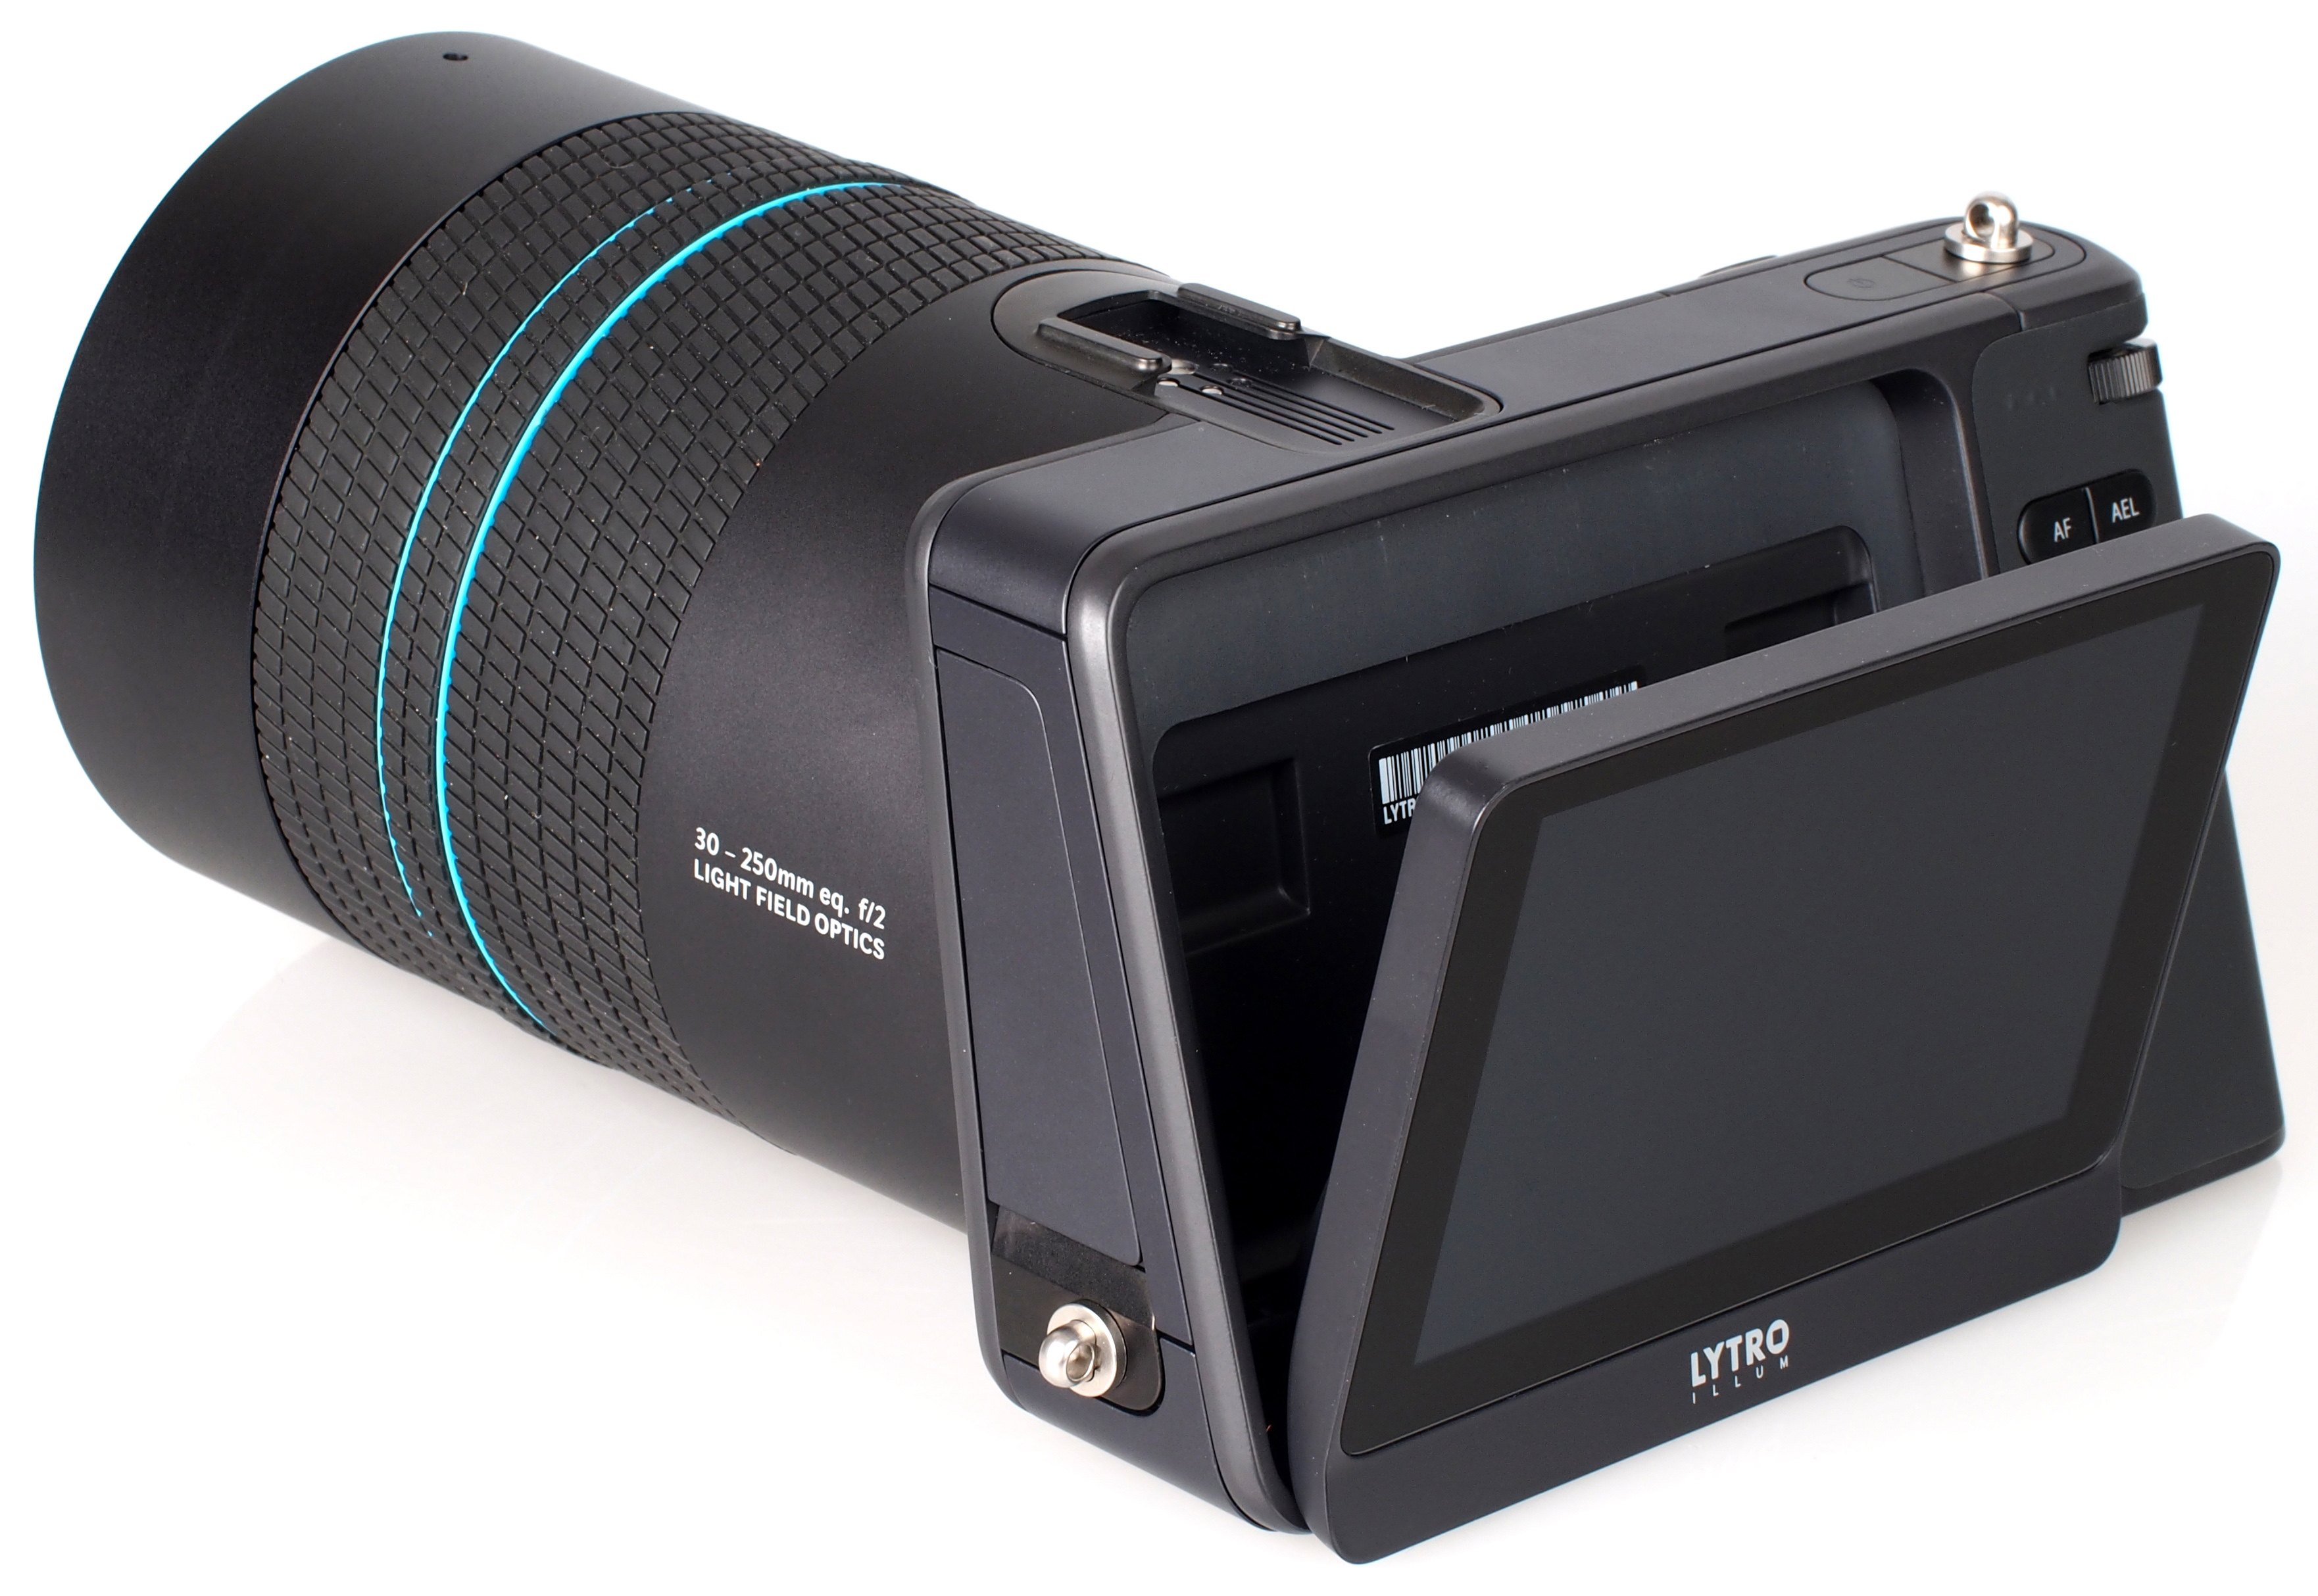
\includegraphics[width=0.8\textwidth]{../../Diagrams/lytro.jpg}
\label{fig:C2S0F3}
\end{figure}
\end{frame}

\begin{frame}{Shearlet Representation of LF (Vagharshakyan et al., 2015)}
\begin{figure}[h!]
\centering
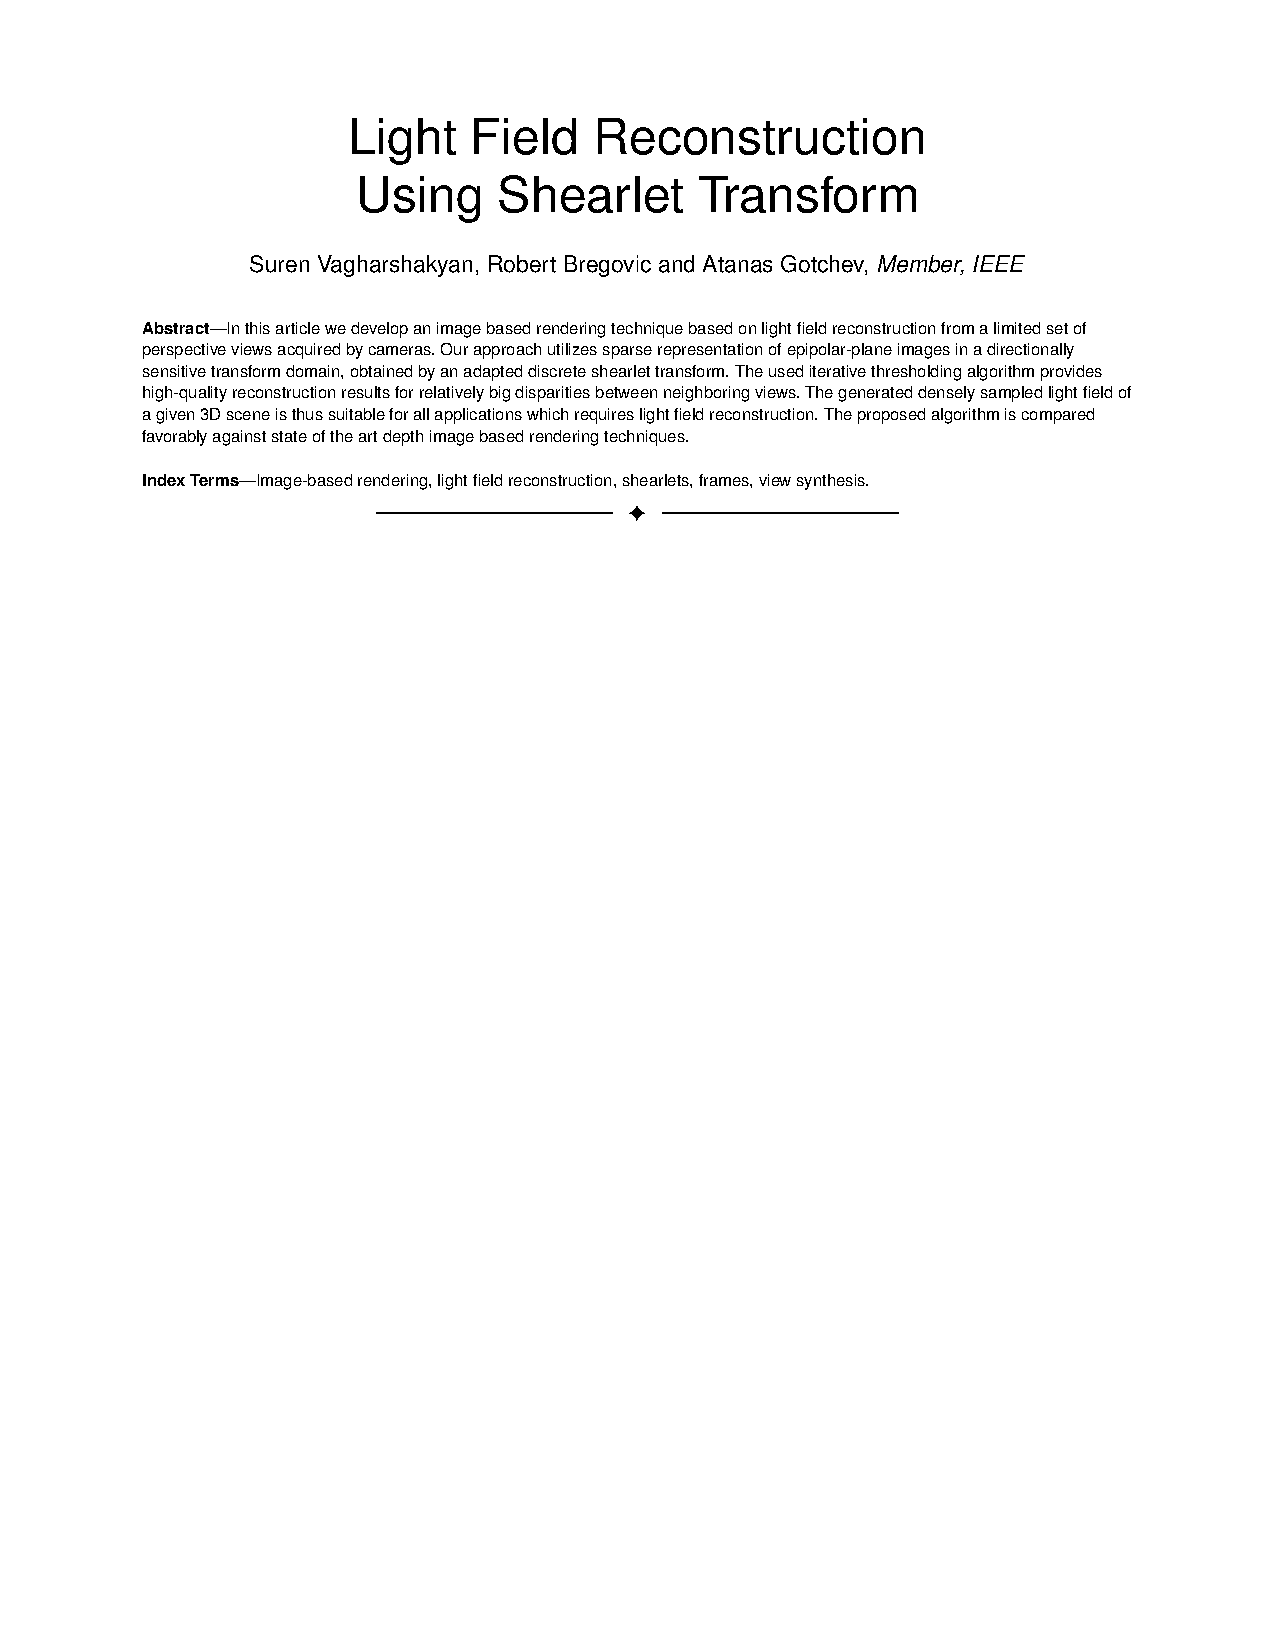
\includegraphics[width=1\textwidth]{./images/LightField_Shearlet.pdf}
\end{figure}
\end{frame}

\begin{frame}{Freedom of knowledge and reproducible research}

\begin{quote}
An article about computational result is \\
advertising, not scholarship. The actual \\
scholarship is the full software environment,\\
code and data, that produced the result.
\end{quote}
\begin{flushright}
\textbf{Buckheit and Donoho (1995)}
\end{flushright}
\end{frame}

\begin{frame}{Stereo Vision and Epipolar Geometry}
\begin{block}{}
\begin{itemize}
\item \textbf{Stereo Vision:} The human brain generates the 3D depth perception of its sorroundings by triangulating the points of a scene using the information coming from both eyes.

\pause
\item \textbf{Epipolar Geometry:} Generalization of Stereo Vision with more than two views, assuming the epipolar constraint.

\pause
\item \textbf{Epipolar Constraint:} Analysis of object position while assuming the knowledge of the camera motion.
\pause
\begin{figure}[h!]
\centering
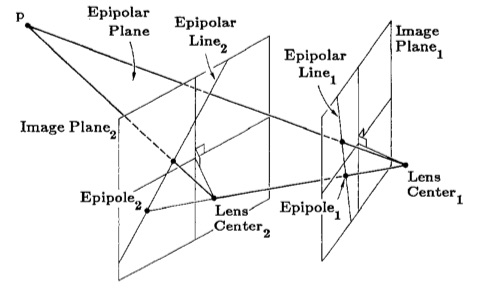
\includegraphics[width=0.52\textwidth]{../../Diagrams/epipolarline.jpg}
\end{figure}
 
\end{itemize}
\end{block}
\end{frame}

\begin{frame}{Epipolar Plane Images (EPIs) on straight line trajectories}
\begin{figure}[h!]
\centering
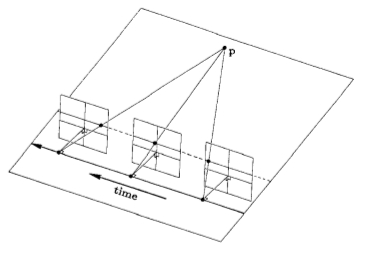
\includegraphics[width=0.45\textwidth]{../../Diagrams/perp-move.jpg}
\end{figure}

\pause
\begin{figure}[h!]
\centering
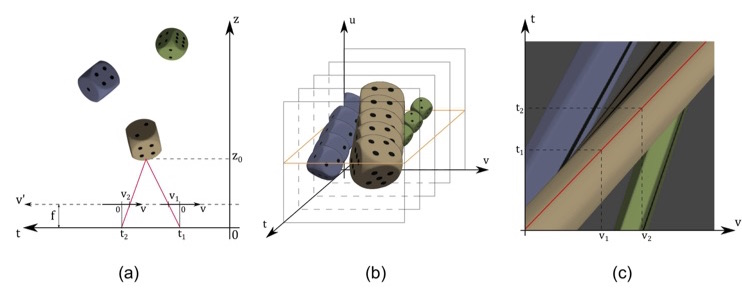
\includegraphics[width=0.90\textwidth]{../../Diagrams/EPI-dices.jpg}
\end{figure}

\end{frame}

\begin{frame}{Functional Analysis of EPIs}

\end{frame}

\begin{frame}{Depth map estimation with EPIs}

\end{frame}

\begin{frame}{Physical acquisition setup}

\end{frame}

\begin{frame}{Computational acquisition pipeline}

\end{frame}

\begin{frame}{Sparse representation and sampling rate}

\end{frame}

\begin{frame}{Reconstruction method with inpaiting}

\end{frame}

\begin{frame}{Cone Adapted Shearlets}

\end{frame}

\begin{frame}{Universal Shearlets and $\alpha$-Shearlets}

\end{frame}

\begin{frame}{Shearlet-based inpainting with iterative hard thresholding}

\end{frame}

\begin{frame}{Line detection and depth map estimation}

\end{frame}

\begin{frame}{Conclusions and Outlook}

\end{frame}

\begin{frame}{Thanks!}
\begin{center}
\Large{Questions?}
\end{center}
\begin{figure}[h!]
\centering
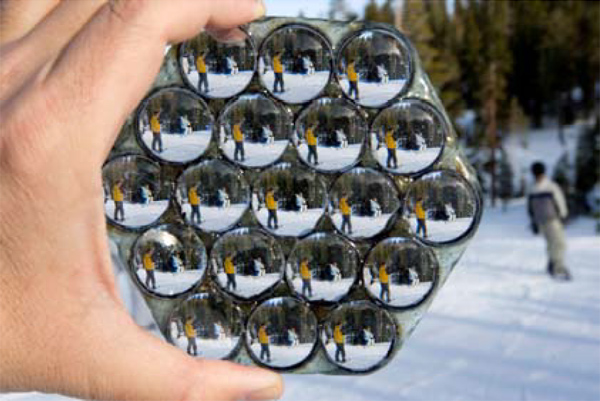
\includegraphics[width=0.8\textwidth]{./Images/lf-camera.jpg}
\end{figure}
\end{frame}

